%----------------------------------------------------------------------------
\chapter{Tervezés}
%----------------------------------------------------------------------------

\section{Szoftver terv}

A rendszer architektúrája a következő komponensekből tevődik össze: felhasználói interfész, backend API, mesterséges intelligencia szolgáltatásai, adatbázis. Ez a több komponenses felépítés működtetéséhez szükséges az internetkapcsolat, amely a kommunikációhoz segít hozzá a komponensek között. A rendszer architektúráját a következő ábra szemlélteti, ahol megfigyelhető a részek közötti kapcsolat és adatáramlás.

\begin{figure}[ht]
    \centering
    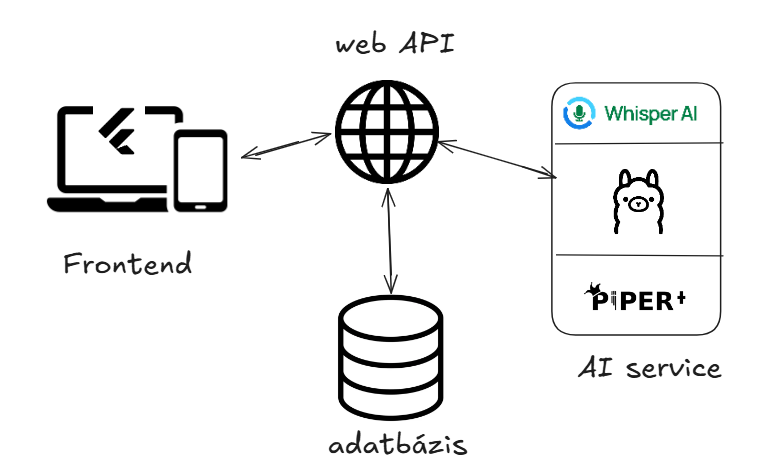
\includegraphics[width=0.8\linewidth]{images/rendszer.png}
    \caption{Rendszer architektúrája}
    \label{fig:arch}
\end{figure}
\newpage

\subsection{Logikai nézet}

A felhasználói felület egy Flutter framework segítségével fejlesztett mobilalkalmazás. Ez lehetővé teszi a cross platform alkalmazások készítését, így az alkalmazásunk amelyet eredetileg mobilra fejlesztettem, könnyedén futtatható weben, akár desktopon is. A felhasználók ezen a területen érhetik el az alkalmazás funkcióit, mint a beszélgetéseket, gyakorló feladatokat, fejlődésükről való statisztikákat.

A backend rétegért a .NET alapú Web API felelős, amely üzleti logikát, autentikációt, adatkezelést, frontend és adatbázis közötti kommunikációt is végrehajt. Az API fogadja a kliens kéréseit, feldolgozza azokat, majd visszaküldi a megfelelő válaszokat.

A rendszer lelke, legfontosabb része: az API szervíz, amely Python alapú réteg. Itt valósulnak meg a mesterséges intelligenciával kapcsolatos funkciók. Ez a komponens felelős többek között a beszédfelismerésért, a nyelvi hibák felismeréséért és javításáért, válasz generálásért, nem utolsó sorban pedig a szöveg felolvasásáért. Az AI szolgáltatások külön komponensekként működnek, amelyekkel a backend API kommunikál. \cite{fowlerMicroservices} Az AI szolgáltatások, amelyek a beszélgetéshez hozzájárulnak azok a Whisper, Phi3, Piper szolgáltatás. A konkrét flow, ami végigmegy ezeken az AI-okon: amikor a felhasználó beszél a mesterséges intelligenciához, akkor a Whisper dolgozza fel a beszédet, amelyet átalakít szöveggé, ezt a szöveget átadja a Phi3 LLM modellnek \cite{whisper,fasterwhisper,phi3,piper}, amely többek között a választ generálja a szövegre, így szimulálva a valós beszélgetést, ezt a választ viszont szövegként adja vissza a Phi3 modellünk, így végezetül a Piper AI modell alakítja át a szöveget hanggá, biztosítva a valós beszélgetés érzetét.

Az adatok tárolásához egy MSSQL adatbázist használunk. Itt kerülnek eltárolásra a felhasználói adatok, beszélgetés címek, hibák, gyakorlási adatok és statisztikák. Az adatbázis kezeléséhez Code First megközelítést alkalmaztam Entity Framework segítségével, amely lehetővé teszi az adatmodellek egyszerű kezelését és migrációk használatát. \cite{efcoreMigrations}

A komponensek közötti kommunikáció internetkapcsolat segítségével megvalósított. A felhasználói felületről érkező kérések először a backend APIhoz kerülnek, amely szükség esetén kommunikál az AI szolgáltatásokkal vagy az adatbázissal. A feldolgozott válasz ezután visszakerül a kliens alkalmazásba.


\subsection{Folyamat nézet}

Az alábbiakban néhány lényeges folyamatot mutatok be, hogy hogyan viselkednek különböző részei a rendszernek.

\begin{enumerate}
    \item \textbf{Hangalapú beszélgetés}
    \begin{itemize}
        \item A felhasználó hangüzenetet küld az alkalmazás számára
        \item A hangfájlt elküldjük az APIn keresztül az AI szolgáltatáshoz
        \item A továbbítás után speech to text AI modell szöveggé alakítja a beszédet
        \item Az AI feldolgozza a szöveges üzenetet, ehhez választ generál és megállapítja a hibákat, amelyeket json formátumban küld vissza az endpointban
        \item A generált választ text to speech AI áltat hanggá alakítjuk, ezt eltároljuk egy mappába
        \item Az elkészült válasz visszakerül a felhasználói felületre és a hang megszólal, de újrajátszható is lesz a hang egy gomb segítségével, és a szavakat is fel lehet mondatni az AI segítségével egy kattintással.
    \end{itemize}
    \item \textbf{Hibák felismerése és eltárolása}
    \begin{itemize}
        \item Amikor a felhasználó az AI modellel beszélget, akkor az AI elemzi a felhasználó válaszai helyességét.
        \item Ha nyelvi hibát észlel automatikusan eltárolja azt a hibák közé, csoportosítja azt, és magyarázatot is generál
        \item Ez majd a gyakorláson alapuló tanuláshoz járul hozzá.
    \end{itemize}
    \item \textbf{Gyakorló feladat generálása}
    \begin{itemize}
        \item A rendszer lekéri a felhasználó hibáit az adatbázisból
        \item A felhasználó tud írásban vagy hangban is gyakorolni, hangban azért nehezebb de hatékonyabb, mert az AI érzékeny az akcentusra és a hanglejtésre is
        \item Gyakorlatilag a felhasználónak ki kell javítani az előzőekben elkövetett hibáit
        \item A felhasználó válaszát az AI javítja ki
        \item Ezen gyakorlatok eredményei eltárolódnak az adatbázisban
        \item Ezek a gyakorlatok hozzájárulnak a felhasználó fejlődéséhez, az eltárolt adatai pedig a statisztikákhoz és mérésekhez
    \end{itemize}
    \item \textbf{Statisztikák frissítése}
    \begin{itemize}
        \item A rendszer a beszélgetések és gyakorlások során különböző adatokat gyűjt a felhasználó aktivitásáról
        \item Ezeket az adatokat az adatbázisban tároljuk el
        \item Az API feldolgozza az adatokat és statisztikákat készít, mint például a hibák száma, gyakorlások száma, fejlődési tendencia
        \item A statisztikák megjelennek a felhasználó profilján és statisztikai felületén
    \end{itemize}
\end{enumerate}

\newpage
\section{Adatbázis terv}

\begin{figure}[ht]
    \centering
    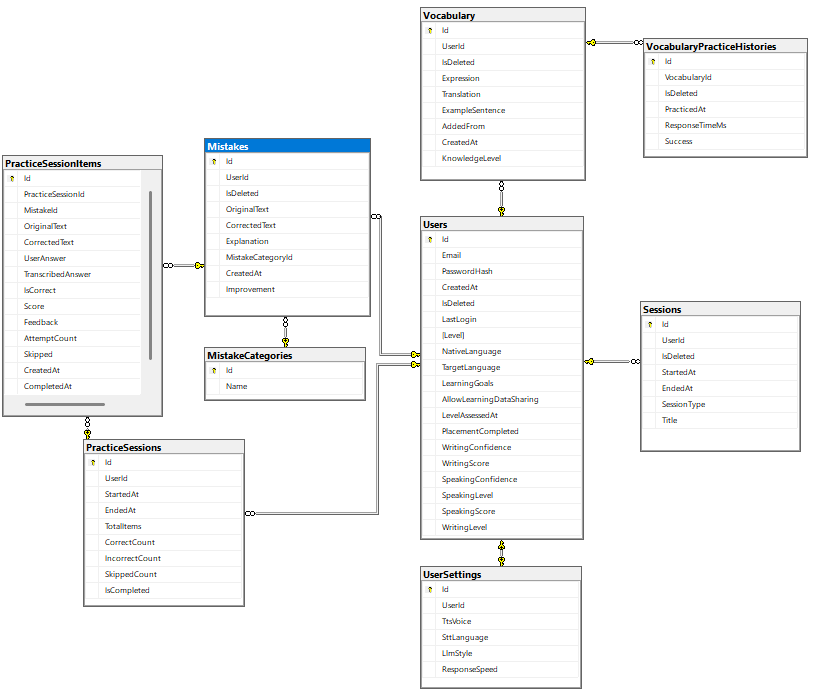
\includegraphics[width=0.8\linewidth]{images/adatbazis2.png}
    \caption{Adatbázis terv}
    \label{fig:database}
\end{figure}
Az adatbázist relációs adatbázisként terveztem meg, amely mindössze 9 táblával rendelkezik. Ezekben a táblákban tárolom el a felhasználó adatait, gyakorlatait. Ezek hozzájárulnak az aplikáció megfelelő működéséhez.

Ezekben a táblákban a legnagyobb a felhasználó adatait tartalmazó tábla, ez egy nagyon fontos hely, amiben sok lényeges adat van eltárolva, ezek mind hozzásegítenek a fejlődés méréséhez és magához a fejlődéshez is, mivel az AI ehhez mérten válaszol neki.

A Vocabulary  táblában mentődik el minden olyan szó vagy szókapcsolat, amelyet a felhasználó nem ismert és ezeknek fordítása. Ezeket a szavakat elmentheti a felhasználó manuálisan, ha bárhol is szembejön vele és szeretne egy olyan helyre menteni, ahol majd előveheti és gyakorolhatja azt, illetve a mesterséges intelligenciával történő beszélgetés során is hozzáadhat ehhez a táblához.
A VocabularyPracticeHistory tábla a Vocabulary-ba eltárolt kifejezések tanulásához járul hozzá. Mivel flashcardok segítségével gyakorolhatja ezeket a felhasználó, itt tárolódik el a helyessége, a válaszidője, és minden más fontos adat, amelyet felhasználhatunk a fejlődés elemzésére.

A Mistakes tábla az azok a szókapcsolatok vagy mondatok tárhelye és azoknak javított verziója, amelyeket a felhasználó elhibázott beszélgetés közben. Mindez úgy tárolódik el ebbe a táblába, hogy beszélgetés közben a mesterséges intelligencia figyeli, milyen hibákat vét a felhasználó és mindezt elmenti kijavított verziójával együtt és magyarázattal. 
Ezeket a hibákat nem hiába mentjük el, ugyanis gyakorló feladatokkal megtanítjuk a helyes verzióját ezeknek. A PracticeSessions és PracticeSessionItems ezért is kapcsolódik a Mistake táblához, mivel a felhasználó gyakorlását ide tároljuk el, minden egyes adatot róla.

A Sessions tábla a mesterséges intelligenciával való beszélgetésről tárol összefoglaló címet, mivelhogy a felhaszálók biztonsága érdekében nem tároljuk a teljes beszélgetést. Ezen kívül még néhány alapvető adat kerül itt tárolásra, mint a beszélgetés kezdete vagy vége.

Az adatbázis MSSQL segítségével íródott. \cite{mssql} Ennek kiválasztásakor a teljesítmény, skálázhatóság és könnyen integrálhatóság volt a szempont. A .NET keretrendszerrel és a Visual Sturdioval nagyon jól integrálható ez, így mindenképp a legjobb választásnak bizonyult.

Az adatbázisterv a \ref{fig:database} ábrán látható.

\section{Felhasználói felület terv}

\begin{figure}[ht]
    \centering
    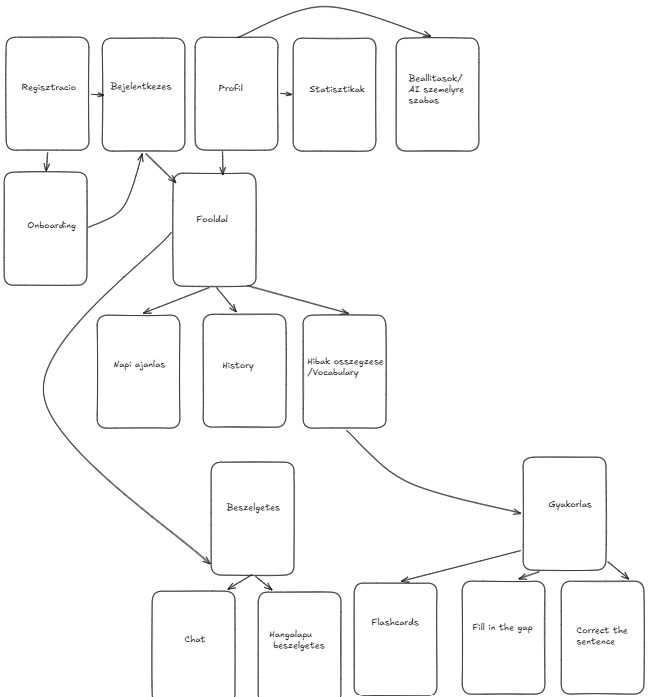
\includegraphics[width=0.8\linewidth]{images/fft.png}
    \caption{Felhasználói felület terv}
    \label{fig:fft}
\end{figure}

A felhasználói felületet tervezéséhez egy egyszerű digitális eszközt használtam. Mivel első sorban nem a felhasználói felület volt számomra a szempont, így inkább egy egyszerűbb tervet készítettem az Excalidraw \cite{excalidraw} alkalmazás használatával. Az alkalmazás fejlesztésénél ezeket vettem elő, ezek biztosították az irányt, amerre haladt a projekt. Néhol újabb dolgokat is beillesztettem fejlesztés közben, nem ragaszkodtam a kezdetleges terveimhez mindig.

A felület tervezésénél nem volt pontos irány, hogy merre rakjuk a gombokat, vagy milyen színeket használjunk, inkább egy átfogó képet szerettem volna kapni az alkalmazásról. Arra fektettem a hangsúlyt a tervben, hogy milyen oldalak, képernyők legyenek az applikációban és a többi részével fejlesztés közben foglalkoztam.

A \ref{fig:fft} ábrán látható a kezdetleges terv, amelyet még az elején a tervezési fázisban készítettem. Itt látható 17 darab képernyő terv és a nyilak jelölik az azok közötti kapcsolatokat. Mára elmondható, hogy a többsége ezeknek a terveknek megvalósult, és hasonlóan sikerült elkészíteni a kapcsolatokat is, mint ahogyan az ábrán látható. Így elmondható, hogy ez a tervezés mindenképpen megalapozta az elkészítés folyamatát.

Ez a tervezés nem csak a felhasználói felület elkészítésében volt hasznomra, hanem a teljes fejlesztés során. Mivel itt a nyilak segítségével megtekinthető a teljes flow, így nem csak a frontend fejlesztésnél, hanem a backend elkészítésénél is rálátást nyertem arra, hogy melyik feature mi után következzen.


\section{Verziókövetés}

A verziókövetés tekintetében a Github volt számomra egy elengedhetetlen választás. Ide mentettem minden elkészített featuret. Fontosnak éreztem a verziókövető rendszer használatát, ugyanis egy összetett rendszerről beszélünk, amelyben a működő komponenseket jó ha eltároljuk valahol és bármi elakadásnál vissza tudjuk húzni a működő verziót. Ez látható a  \ref{fig:github} ábrán. \cite{gitVersionControl}

Egy repository segítségével kezeltem a projektet, amelyben három nagy komponens szerepel: a backend, frontend és az ai service. 

\begin{figure}[ht]
    \centering
    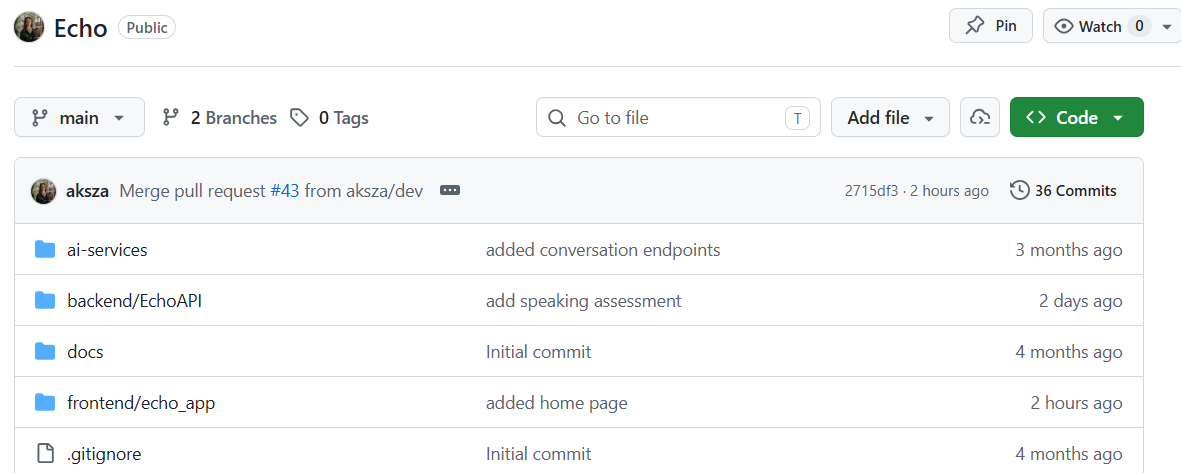
\includegraphics[width=0.9\linewidth]{images/git.png}
    \caption{Verziókövető rendszer}
    \label{fig:github}
\end{figure}

A hatékony programozáshoz készítettem egy branchet is, hogy a main branch tisztán maradhasson mindig, és a csak a működő feature komponensek legyenek itt, ne a félkészek. A dev branchen fejlesztettem mindent. Itt több commit is volt készítve minden featurehöz. Amikor sikerült elkészíteni egyet, pull request lett nyitva, itt mégegyszer megvizsgáltam a kódot, ha találok benne hibát. Amikor jónak tűnt, máris befésültem a mainre.Ezzel a megközelítéssel könnyedén és tisztán ment a fejlesztés. A branch ábrája a \ref{fig:branch} megtekinthető.


\begin{figure}[ht]
    \centering
    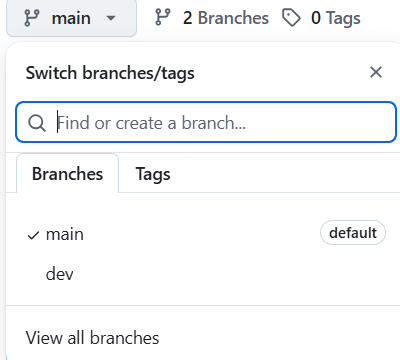
\includegraphics[width=0.4\linewidth]{images/branch.png}
    \caption{Branch-ek}
    \label{fig:branch}
\end{figure}

\section{Projektmenedzsment}

Próbáltam úgy megoldani a projektmenedzsmentet is, hogy azonos platformon legyen a verziókövetőnkkel. Így esett arra a választás, hogy a Github issues menüpontját használjam. \cite{githubIssues} Ez arról szól, hogy minden feature számára nyitok egy issue-t. Az issue-k tartalmazhatnak subissue-kat is, ha túl nagy issue jött létre. 

Ez számomra azért volt a legkézenfekvőbb, mivel egy platformon elérhetem a kész kódot, a feature terveket és pull request formájában a már kész, elfogadásra váró feature-öket. 

A flow az volt, hogy a tervezés résznél megírtam itt, issue formájában minden egyes feature-t, amelyet le kell implementálni. Ekkor meg lehetett itt adni, hogy ki kell elkészítse ezt - ez nagyobb csapat esetében nagyon hasznos lehet, de nálam értelemszerűen én voltam megjelölve itt. Ezután labelt, milestone-t is lehetett hozzáadni, viszont én az egyszerűség kedvéért ezeket a részleteket hanyagoltam. Miután elkészült a tervezés részben az összes issue, kezdődött a fejlesztés. Kiválasztott feature-t leimplementáltam, ezután pedig pull requestet nyitottam. Itt méginkább bebizonyosodott, hogy jó választás volt az, hogy ugyanazon a platformon verziózok és menedzselem a projektet is, ugyanis van egy olyan funkció, hogy a pull request leírásában ha hivatkozunk az adott issue-ra, akkor a pull request merge végrehajtása után automatikusan lezárja az issue-t. Így nem kellett manuálisan lezárnom minden elkészített feature-höz tartozó issue-t.

Az Github oldalán pedig bármikor megtekinthetőek voltak a nyitott vagy már lezárt issue-k. Ezeket bármikor újra lehetett nyitni, vagy akár a nyitottakat lezárni, duplikáltnak jelölni. Úgy gondolom, hogy ez egy olyan projekthez, amit egy személy készít, bőven elegendő projektmenedzsment eszköznek, mivel minden szükséges kellék megvan benne.

\newpage

\begin{figure}[ht]
    \centering
    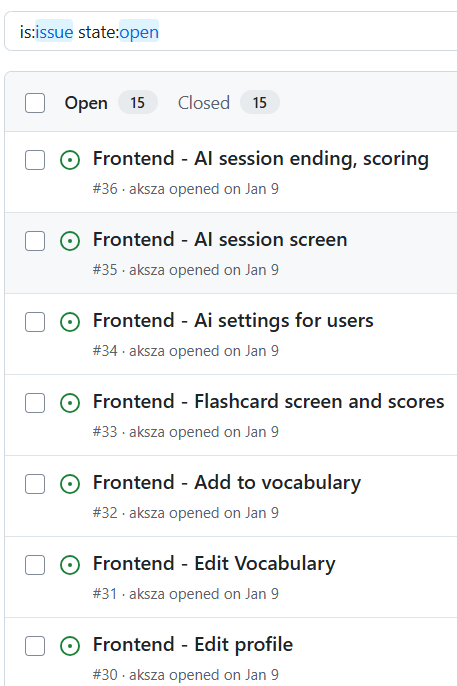
\includegraphics[width=0.5\linewidth]{images/issues.png}
    \caption{Projektmenedzsment}
    \label{fig:projectmanagement}
\end{figure}